\setchapterpreamble[u]{%
    \margintoc\hfil
    \dictum[Richard Feynman]{What I cannot create,\\I do not understand.}
}

% Methods
\chapter{The spectrometer}
\labch{methods}
% Write in theorem-proof fashion

The individual parts of the spectrometer have been designed with several goals in mind. The main guiding principle was reproducibility and availability such that anyone can reproduce the build with minimal effort. All the necessary steps are documented below, including the reasoning for steps not taken. For verification and testing of the parts below the console (see \refsec{console}) itself may be used\sidenote{Instruction for using the RedPitaya as an \gls{lcrmeter}, \acrshort{vna}, or spectrum analyser can be found in its documentation}. A more practical solution is using separate devices for this to avoid the reconfiguration hassles. The open-source NanoVNA-H4\sidenote{\approx{}60CHF, \url{https://nanovna.com/}} \acrshort{vna} and the tinySA\sidenote{\approx{}50CHF, \url{https://tinysa.org/}} spectrum analyser are affordable and at these frequencies very capable alternatives to expensive lab equipment. They have been used extensively during the development of the hardware.

The following sections describe the design and build process --- including the reasoning behind the decisions taken --- of the \magnethical{} NMR spectrometer. \reffig{block-diagram} shows an overview schematic of the main components that will be discussed.

In general, the components were selected to be standard parts wherever possible. RF electronics are highly sensitive to stray capacitances and inductances, therefore most dedicated RF components use surface mount\sidenote{as opposed to through-hole (SMT)} (SMD) technology, sometimes even without pins. The passive components, like inductors, capacitors and resistors are in 0805\sidenote{0805 means \qty{0.08}{in} x \qty{0.05}{in}. PCB design is a mess of different unit systems, e.g. board sizes are often given in \unit{\milli\metre} whereas trace width is often given in \unit{mil} (thousandth of an \unit{in}). Rarely 0805 is written as 2012M: \qty{2.0}{\milli\metre} x \qty{1.2}{\milli\metre}} sizing, which was deemed large enough to be still easy to solder by hand. All traces were impedance matched to \qty{50}{\ohm} on standard \qty{1.6}{\milli\metre} FR4 cards, milled with standard drill sizes to facilitate the use of affordable standard manufacturing processes. Lastly, SMA connectors were chosen for their small footprint and secure screw connection, as opposed to BNC connectors (large) and SMB connectors (less secure connection). Most parts were searched for using the parametric search functionality of the big distributors and filtered for only active, available and stocked parts --- a rather large restriction in times of a global chip shortage.

\begin{figure}[hbt]
    \centering
    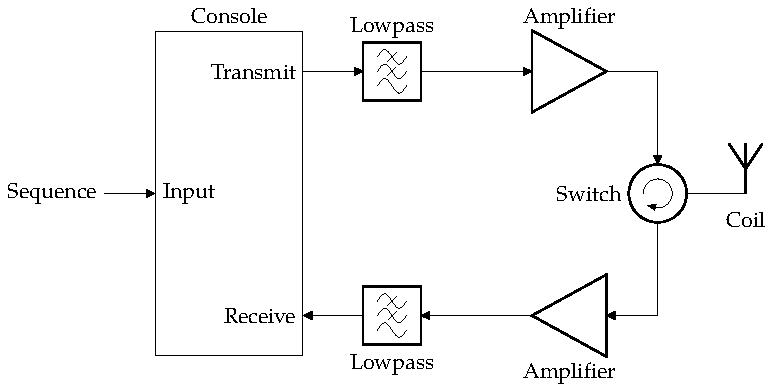
\includegraphics{images/block_diagram.pdf}
    \caption{\captiontitle{Block Diagram.} The main components of the \magnethical{} NMR spectrometer, including the console, lowpass filters, analogue amplifiers, transmit-receive switch and transmit-receive coil.}
    \labfig{block-diagram}
\end{figure}

The section order follows the path of the signal, that is, clockwise around the schematic starting with the console.

\section{The console}
\labsec{console}
\begin{marginfigure}[-4.5\baselineskip]
    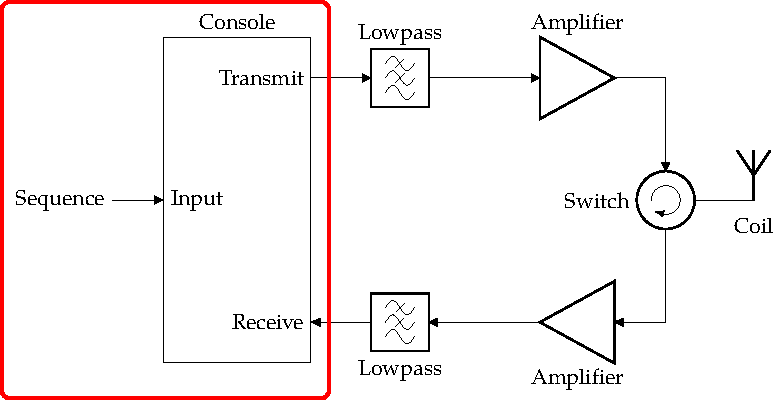
\includegraphics{block_diagram_highlight_console.pdf}
    \labfig{block-diagram-console}
\end{marginfigure}

The relatively low frequency of \(f_0 = \qty{25}{\mega\hertz}\)\sidenote{Given by the \ch{^1H} resonance frequency in the \qty{0.6}{\tesla} magnet} as well as the low bandwidth of only about \qty{10}{ppm}\sidenote{Equals \qty{25}{\hertz} at \qty{25}{\mega\hertz}} of the expected signal allows moving a lot of previously analogue tasks into the digital domain, greatly simplifying the hardware setup and making it more flexible. According to the Nyquist theorem, the minimum frequency that can be used to digitize an analogue signal without loss of information\sidenote{That is, without aliasing issues} must be more than twice as large as the highest frequency component of interest in the signal. In our case, the analogue-to-digital conversion must happen with more than
\[
    f_{min} \ge 2f_0 = \qty{50}{\mega\hertz}
\]
if oversampling is to be used. The setup could also make use of the low bandwidth of the signal and use the aliasing effect of the analogue-to-digital conversion to its advantage using undersampling. Since this requires taking further care when sampling and filtering, and the expected frequencies are low enough to make oversampling feasible, oversampling is employed in this setup. This has the added advantage of higher flexibility since the sampling frequency can be easily adjusted downwards.

For digital processing, a \acrfull{fpga} is used, which can be thought of as a piece of programmable hardware. To ease development a ready-made \acrshort{fpga} board --- the RedPitaya SDRlab 122-16 shown in \reffig{redpitaya} --- was chosen. With a sampling frequency of \qty{122.88}{\mega\sample\per\second} it is well above the Nyquist limit. Combined with a resolution of \qty{16}{bit} it is more than capable of capturing all relevant data from the analogue signal. Due to the commercial nature, the board is easily procured directly from RedPitaya or any of the well-known distributors\sidenote{For example Digikey, Mouser, Farnell, \dots}. A possible open-source alternative in the future would be the LimeSDR\sidenote{\url{https://limemicro.com/products/boards/limesdr/}}. With a sampling frequency of \qty{61.44}{\mega\sample\per\second}, limited by the USB3 interface, and a resolution of \qty{12}{bit} it is less powerful than the RedPitaya, but still fast enough for oversampling without loss of information. This board would cost less than half (\approx 280CHF) of the RedPitaya board and would enable a completely open design of the spectrometer --- in line with the accessibility goals of this work. Unfortunately, due to the young age of this project and the crowd-sourced nature, no board was available for purchase at the time of writing.

\begin{figure}[hbt]
    \centering
    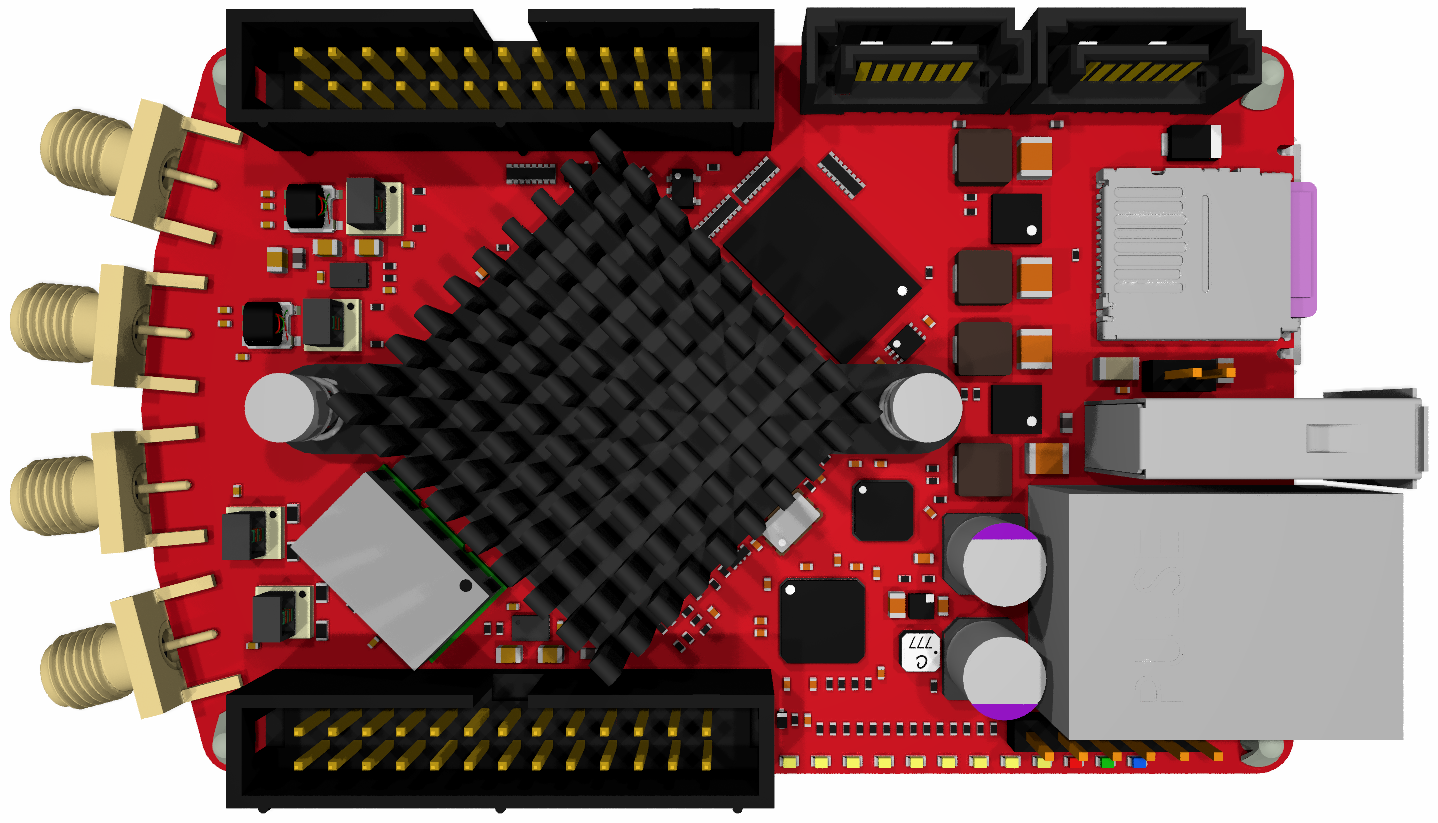
\includegraphics{images/rp122-16.png}
    \caption{\captiontitle{RedPiaya SDRlab 122-16.} 3D rendering of the console in KiCAD. Can be thought of as an \enquote{RF Raspberry Pi}. It has a Dual Core ARM Cortex A9, \qty{512}{\mega\byte} RAM, Gigabit Ethernet, 2x transmit, 2x receive, an ADC sample rate of \qty{122.88}{\mega\sample\per\second}, \qty{16}{\bit} resolution, a bandwidth of \qty{300}{\kilo\hertz} to \qty{550}{\mega\hertz} and a voltage range of \qty{0.5}{Vpp}/\qty{-2}{\deci\belm} (\qty{50}{\ohm}). The DAC has the same sample rate and voltage range, but a resolution of \qty{14}{\bit} and a bandwidth of \qty{300}{\kilo\hertz} to \qty{60}{\mega\hertz}.}
    \labfig{poweramp}
\end{figure}

After sampling the signal is demodulated using a quadrature detection system by multiplying it with the signal of a complex numerically controlled local oscillator. The same principle is applied inversely on the sending side for modulation. The resulting complex demodulated signal is then passed through a \acrfull{cic} filter for low-pass filtering and decimation to filter out high-frequency components of the signal and reduce the size of the data stream. The full data steam would incur a bandwidth of
\[
    \qty{16}{\bit} \cdot \qty{122.88}{\mega\sample\per\second} = \qty{245.76}{\mega\byte\per\second}
\]
per channel. With potentially 2 transmit and 2 receive channels this results in a data rate of close to \qty{1}{\giga\byte\per\second}, which is way higher than the theoretical limit of \qty{116}{\mega\byte\per\second} of the Ethernet interface. Due to inefficiencies in the Linux kernel of the RedPitaya Image, the practical data rate limit for continuous streaming is a lot lower at about \qty{20}{\mega\sample\per\second}\sidenote{According to the official \gls{lcrmeter} documentation (\url{https://redpitaya.readthedocs.io/en/latest/appsFeatures/applications/streaming/appStreaming.html})}. This has been improved in Pavel Demin's kernel image, where speeds up to \qty{80}{\mega\byte\per\second} have been measured\sidenote{\url{https://pavel-demin.github.io/red-pitaya-notes/alpine/}}. However, this only becomes relevant on long acquisition times over several seconds and has not been thoroughly tested as it has not been relevant, yet.

All of these digital signal-processing tasks are performed by the \acrshort{marcos} \acrshort{fpga} firmware developed by Vlad Negnevitsky\sidecite{negnevitskyMaRCoSOpensourceElectronic2023}. The system is designed for a low-field MRI system but could be easily adapted for NMR spectroscopy. The demodulated, filtered and decimated data from MaRCoS is then sent through its C server to the developed high-level Python interface. \reffig{marcos} shows an overview of the \acrshort{marcos} architecture. For more information on the Python programming interface see \refsec{software}.

\begin{figure}[hbt]
    \centering
    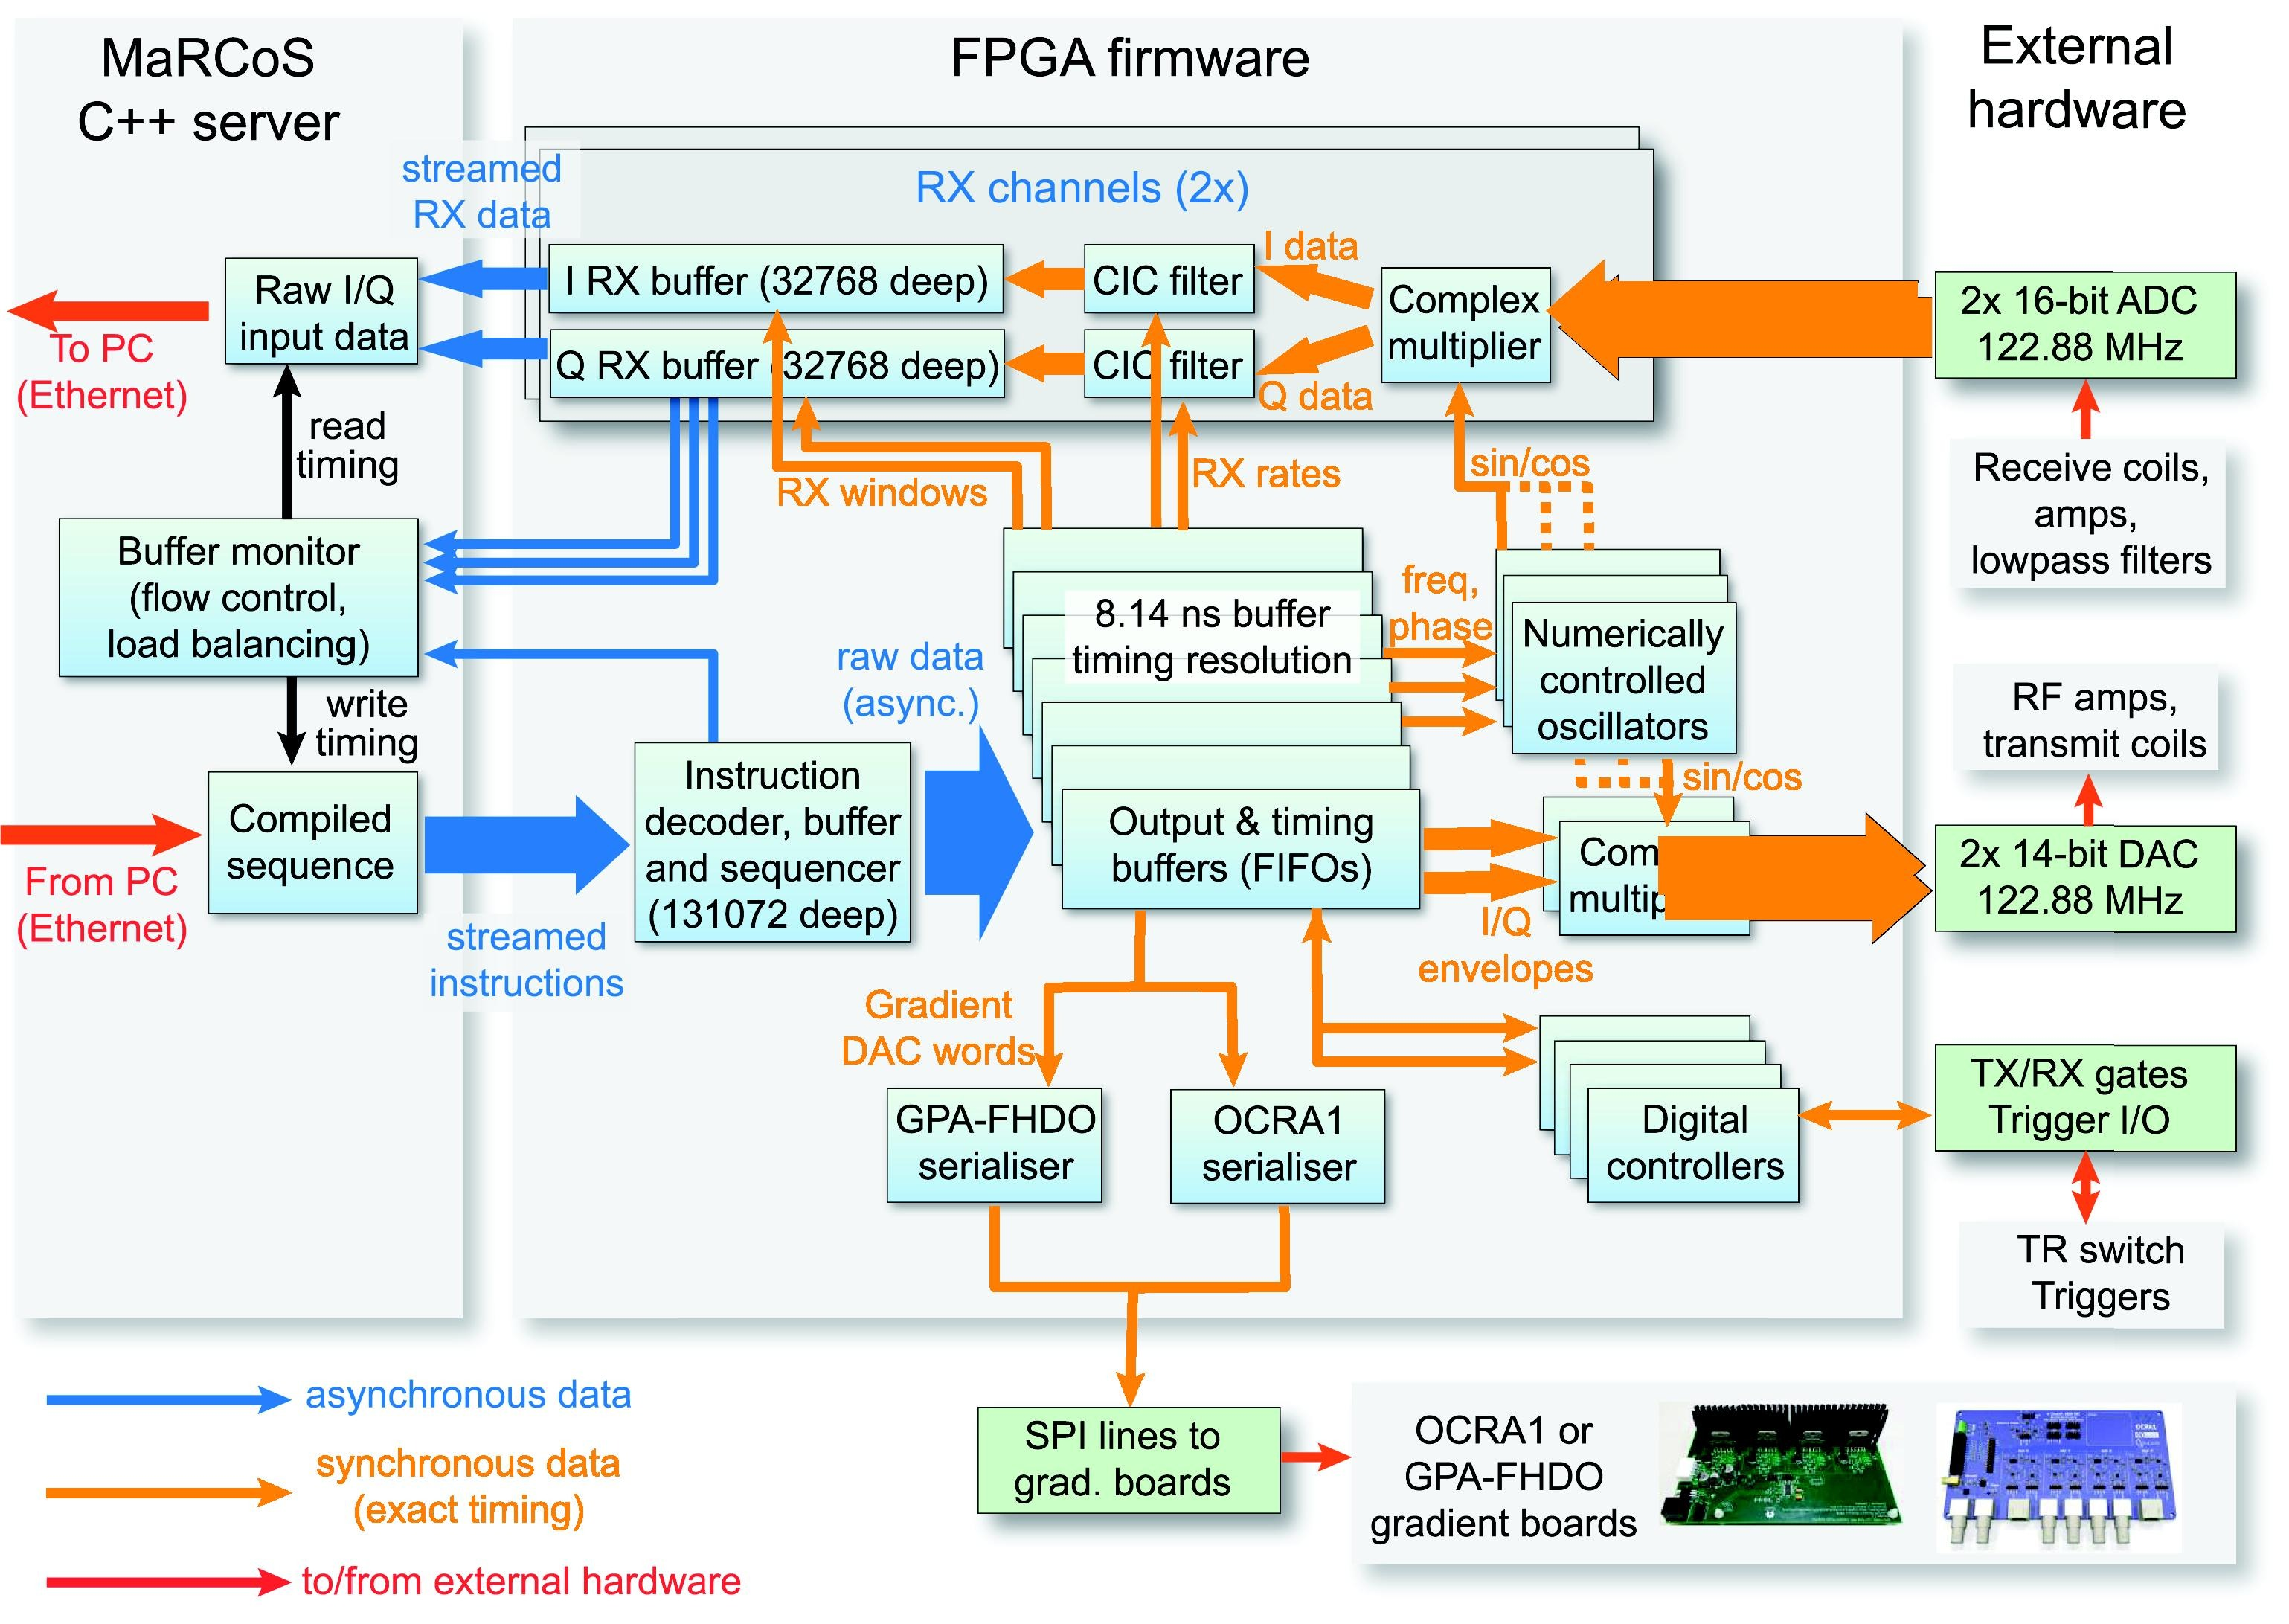
\includegraphics{images/marcos.jpg}
    \caption{\captiontitle{MaRCoS system architecture.} \enquote{The server receives a sequence from the client PC via Ethernet and streams it to the FPGA firmware, where it is translated into time-synchronous hardware operations including RF and gradient outputs. The firmware receives data from the ADCs, demodulates and filters it, and saves it into RX buffers, from which it is read by the server and sent to the PC} \cite{negnevitskyMaRCoSOpensourceElectronic2023}, Figure 3}
    \labfig{marcos}
\end{figure}

\todo{Protection diodes, incl. graphs and measurements}

\section{The power amplifier}
\labsec{poweramp}
\begin{marginfigure}[-4.5\baselineskip]
    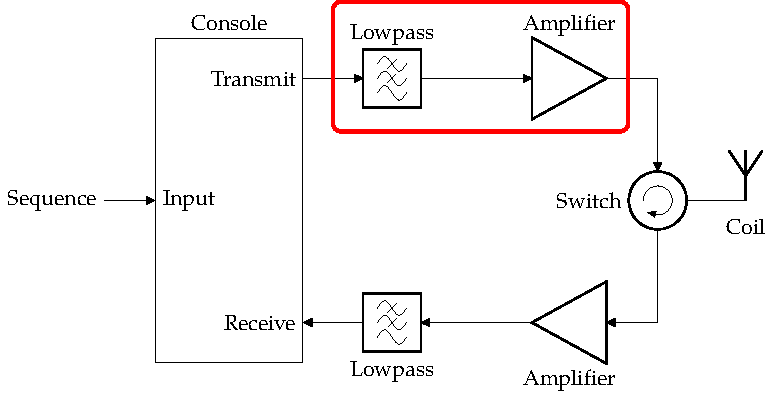
\includegraphics{block_diagram_highlight_tx.pdf}
    \labfig{block-diagram-pa}
\end{marginfigure}

The power amplifier has to amplify the low-power digitally synthesised signal from the console. The console described in \refsec{console} above has a maximum output power of \qty{0.5}{\volt} or \qty{-2}{\deci\belm} into a \qty{50}{\ohm} load.

The output power required to excite a volume of \qty{1}{\centi\meter\cubed} on a bandwidth of about \qty{10}{\kilo\hertz} or \qty{20}{ppm} in a high field magnet (\qty{500}{\mega\hertz} (\ch{^1H})/\qty{11.7}{\tesla}) is about \qty{11}{\watt} \sidecite{louis-josephDesigningBuildingLowcost2019}. The magnet in this work (see \refsec{magnet}) has a field strength of \qty{25}{\mega\hertz} (\ch{^1H})/\qty{0.6}{\tesla}, therefore \qty{20}{ppm} equals an excitation bandwidth of only \qty{500}{\hertz}. The sample Volume is only \(\qty{100}{\micro\litre} = \qty{0.1}{\centi\meter\cubed}\) as well, reducing the required energy further.

Targeting a pulse length of \qty{20}{\micro\second} for a \ch{^1H} \(\frac{\pi}{2}\)-pulse the RF pulse needs to generate a magnetic field of about
\[
    B = \frac{\alpha}{\gamma\tau} = \frac{\frac{\pi}{2}}{\qty{42.577}{\mega\hertz\per\tesla}\cdot{}\qty{20}{\micro\second}} = \qty{1.845}{\milli\tesla}
\]

The magnet has a homogenous region of \(\qty{100}{\micro\litre}\) for a \qty{5}{\milli\meter} NMR tube, resulting in an NMR active length of about \(l = \qty{6}{\milli\meter}\). If we assume a simple solenoid of that length with about \(n = 20\) turns, a Q factor of 100 (usually in the range of 10 to 1000 \sidecite{mispelterNMRProbeheadsBiophysical2015}) and a self-inductance of \(L = \frac{\mu_0n^2A}{l} = \qty{3}{\micro\henry}\)\sidenote{} we can roughly estimate the required peak power \(P\) with the following formulas \cite{mispelterNMRProbeheadsBiophysical2015}
\begin{align}
    B & = \frac{\mu{}_0nI}{l}              \\
    P & = R\underbar{I}^2 = R\frac{I^2}{2} \\
    Q & = \frac{L\omega}{R}                \\
\end{align}
where \(B\) is the magnet field produced by the current \(I\) through a solenoid of length \(l\) with \(n\) windings and and air core of permittivity \(\mu{}_0\). \(P\) is the maximum power pushed into the solenoid by current \(I\) over resistance \(R\) and \(Q\) is the definition of the quality factor for a self-inductance \(L\) and resistance \(R\). Putting it all together results in an estimated power level of
\begin{align}
    P & = \frac{B^2l^2L\omega}{2\mu{}_0^2n^2Q}                                                                                                                                              \\
      & = \frac{(\qty{1.845}{\milli\tesla})^2 \cdot (\qty{6}{\milli\metre})^2 \cdot \qty{3}{\micro\henry} \cdot 2\pi{} \cdot \qty{25}{\mega\hertz}}{2 \cdot \mu{}_0^2 \cdot 20^2 \cdot 100} \\
      & = \qty{457.12}{\milli\watt}
\end{align}

The exact power required is difficult to calculate at best due to various losses of the materials, the sample, the surrounding materials and losses due to radiation. Previous works with low-field NMR spectrometers used power amplifiers with a maximum power output of \qty{1}{\watt}\cite{chenUltralowCostNMR2015} and \qty{5}{W}\cite{louis-josephDesigningBuildingLowcost2019}. Lower power RF amplifiers have the advantage of lower required voltages, lower noise, less cooling requirements and simpler integrated designs.

The most affordable option for the power amplification would be based on \acrshort{rf} transistors. Unfortunately, this also necessitates an involved design process including not only biasing and feedback design, but also impedance matching and power supply circuits of a possible multi-stage power amplifier. This alone could be the topic of another thesis. Therefore, an \acrshort{mmic} approach has been chosen. Furthermore, availability in the \qty{1}{\watt} range is large due to a large commercial market in this power range especially for CATV amplifiers. Therefore, a \qty{1}{\watt} \acrshort{mmic} amplifier was chosen.

The \acrfull{mmic} amplifier has biasing, possible feedback and stabilization requirements all integrated on a single substrate design. In an application-only power, \acrshort{dc} blocking and adequate cooling have to be supplied since this is a Class A amplifier design.

The final board can be found in \reffig{poweramp}, with its schematic in the appendix \refsec{poweramp-schematic} and the part list in \refsec{poweramp-parts}.

\begin{figure}[hbt]
    \centering
    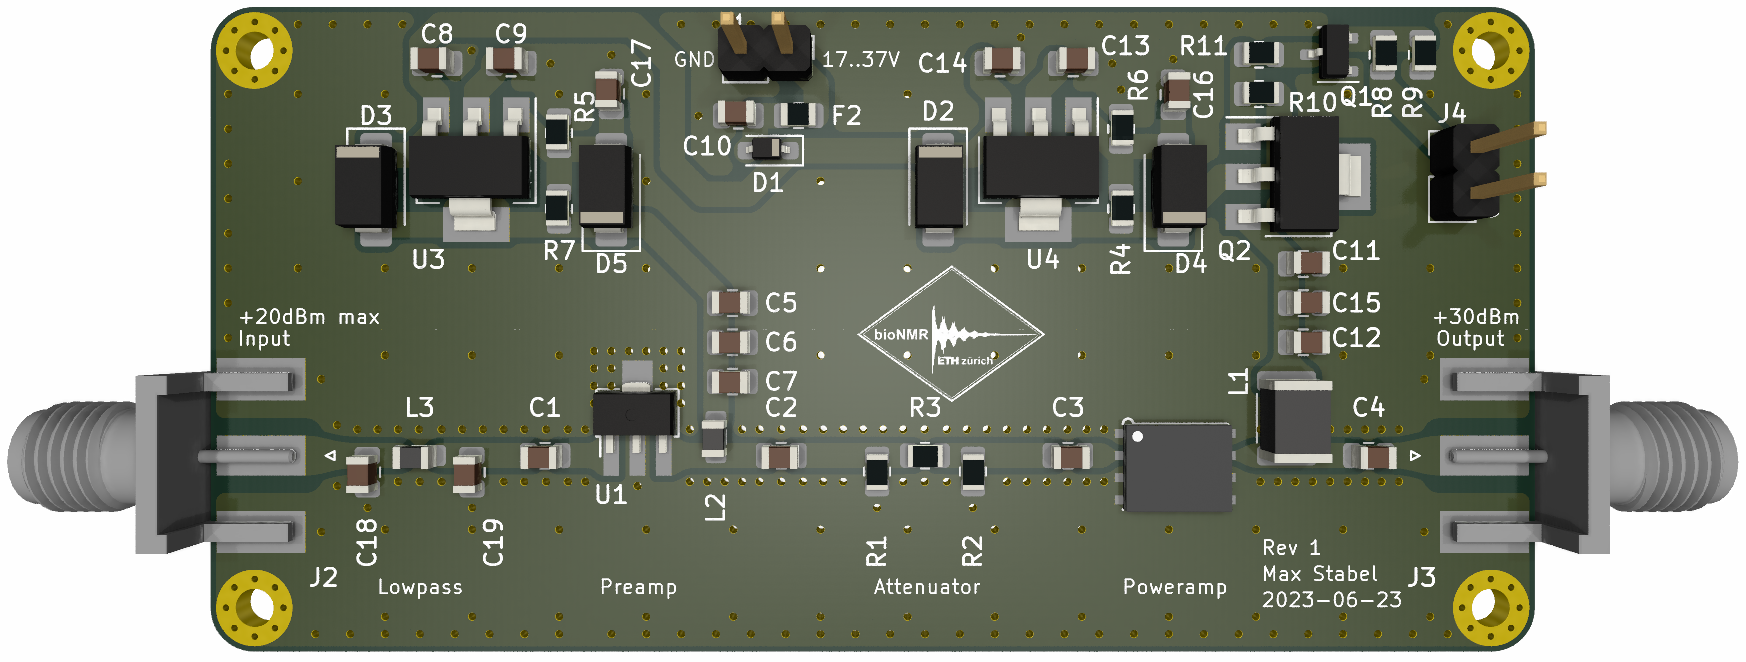
\includegraphics{images/poweramp.png}
    \caption{\captiontitle{\acrshort{rf} power amplifier.} 3D rendering of the power amplifier \acrshort{pcb} in KiCAD. The signal travels from left to right with the power supply circuitry above. It contains two \acrshort{mmic} amplifier stages, the AD5536 and the PHA-202+. A \qty{-6}{\deci\bel} attenuator was added in between and a passive low-pass filter in front (\(f_c = \qty{35}{\mega\hertz}\)). \(G \approx \qty{32}{\deci\bel}\), \(P_{\qty{1}{\deci\bel}} \approx \qty{+30}{\deci\belm}\)}
    \labfig{poweramp}
\end{figure}

The signal from the RedPitaya travels left to right through a low pass, the pre-amplifier, an attenuator and the power amplifier. The parts at the top of the board are standard linear voltage regulators used for stabilizing the voltage from the external DC supply. The power amplifier chip itself can be switched off by cutting the voltage supply.

The low-pass input filter functions as a digital reconstruction filter, smoothing the digitally synthesised waveform by filtering out high-frequency components of the signal left over from the switching of the FPGA and the zero-order hold DAC chip. It is a passive Chebyshev low-pass LC ladder filter realized with three 0805-sized SMD components.

The power amplifier is a PHA-202+, chosen for its easy powering requirements, \qty{50}{\ohm} matching and wide availability. However, it does not have enough gain (\qty{18.3}{\deci\bel})) to take the signal from \qty{-2}{\deci\belm} all the way to \qty{+30}{\deci\belm}. The missing \qty{14}{\deci\bel} in amplification are provided by the preamp (\qty{20}{\deci\bel}) minus the following attenuator (\qty{6}{\deci\bel}).

The AD5536 pre-amplifier is a \qty{50}{\ohm} matched, widely available \qty{20}{\deci\bel} gain GaAs gain block from Analog Devices. It is in an easy-to-solder package and has a low enough frequency specification to work with \qty{25}{\mega\hertz}. Alternatives with this gain and power are often difficult to solder due to the leadless design, unmatched (e.g. AFIC901N) \qty{75}{\ohm} matched (e.g. MAAL-011139) and often cannot amplify such a slow signal (e.g. TAT7430B, starting at \qty{50}{\mega\hertz}).

The \qty{6}{\deci\bel} resistive attenuator in between the amplifiers is realized as a \(\pi\)-circuit similar to the low pass ladder filter. It is used to stabilize the adjacent amplifiers and will dampen any oscillations that might occur due to load or stray capacitances or inductances. If necessary the attenuation could be reduced to e.g. \qty{3}{\deci\bel} to increase the maximum power output of the amplifier, however, since the \(P_{\qty{1}{\deci\bel}} = \qty{29}{\deci\belm}\) for the PHA-202+ it will not grow linearly. The potential distortions should be of little consequence for the transmission signal.

For blocking the DC bias current for the amplifiers simple 0805 100nF caps are used in series as a high pass filter. For a \qty{50}{\ohm} system we can calculate the minimum value for the capacitors using the standard formula \(X_C = \frac{1}{2\pi{}fC}\) and keeping in mind that the block is loaded on both sides thus \( 2 \cdot \qty{50}{\ohm} = \qty{100}{\ohm}\). For \qty{25}{\mega\hertz} we thus get a minimum capacitance of
\[
    C = \frac{1}{2\pi{}fX} = \frac{1}{2\pi{} \cdot{} \qty{25}{\mega\hertz} \cdot{} \qty{100}{\ohm}} = \qty{63.7}{\pico\farad}
\]
The chosen \qty{100}{\nano\farad} are significantly larger and simply chosen for convenience and availability. Their high-pass cut-off frequency is at
\[
    f = \frac{1}{2\pi{}XC} = \frac{1}{2\pi{} \cdot{} \qty{100}{\ohm} \cdot{} \qty{100}{\nano\farad}} = \qty{15.9}{\kilo\hertz}
\]
For the chosen capacitors\sidenote{C0805C104J5RACTU} by KEMET this can be easily verified using the provided K-SIM simulator\sidenote{\url{https://ksim3.kemet.com/capacitor-simulation}}, which confirms an insertion loss (S21) of \qty{0}{\deci\bel} and an input reflection (S11) of \qty{-68}{\deci\bel} for \qty{25}{\mega\hertz}.

\section{The switch}
\begin{marginfigure}[-4.5\baselineskip]
    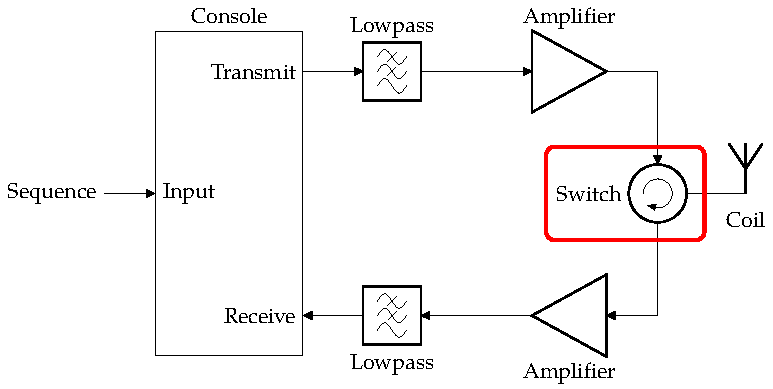
\includegraphics{block_diagram_highlight_switch.pdf}
    \labfig{block-diagram-switch}
\end{marginfigure}

The switch has two main functions:
\begin{enumerate*}
    \item Protecting the receive path from the high power pulses when transmitting and
    \item blocking the noise of the transmit power amplifier when receiving.
\end{enumerate*}
The simplest approach for the user would be a passive switch, that does not need an active signal and simply forwards everything from the transmit port to the probe and everything from the probe to the receive port and nothing else. The possibly most popular design is the passive switch presented in \sidecite{loweFastRecoveryProbe1968} and pictured in \reffig{passive-switch-schematic}. It is based on easy-to-build, cheap and passive. On the downside, it has a narrow bandwidth, which is not a problem for our case, as the resonance frequency of the permanent magnet is fixed and varies only slightly.

\begin{figure}[hbt]
    \centering
    \begin{circuitikz}
        \ctikzset{
            diode=empty,
            diodes/scale=0.8
        }
        \draw[nodes={align=center}]

        % tx diodes
        (0,0) node[left]{Transmit} to[short,o-*] ++(1,0) coordinate(tx)
        (tx) -- ++(0, 0.5) to[D] ++(1.5,0) -- ++(0,-0.5)
        (tx) -- ++(0,-0.5) to[D,invert] ++(1.5,0) -- ++(0, 0.5)
        to[short,*-] ++(1,0) coordinate(mid)

        % A/B
        (mid) node[below](A){A}
        (mid) to[short,*-o] ++(0,2) node[above]{Probe}
        (mid) -- ++(3,0) coordinate(b)
        (b) node[above](B){B}

        % rx diodes
        (b) to[short,-*] ++(0,-0.5) coordinate(rx)
        (rx) -- ++(-0.5,0) to[D] ++(0,-1.5) -- ++(0.5,0)
        (rx) -- ++(0.5,0) to[D,invert] ++(0,-1.5) -- ++(-0.5,0)
        to[short,*-] ++(0,-0.5) node[ground]{}

        (b) to[short, *-o] ++(1,0)
        node[right]{Receive}
        ;
        \draw[<->] (A.east |- B.west) -- (B.west);
        \draw ($(A.east|-B.west)!0.5!(B.west)$) node[above]{\(\frac{\lambda}{4}\)};
    \end{circuitikz}
    \caption{\captiontitle{The passive switch.} Based on Diodes and \acrshort{rf} properties, the passive switch forwards the signal based on signal power. Due to the diode characteristics, the switch leaks up to \qty{0.7}{\volt} without attenuation --- including noise.}
    \labfig{passive-switch-schematic}
\end{figure}

The passive switch's working principle is based on the diode's characteristic to only start conducting above \qty{0.7}{\volt} forward bias and \acrshort{rf} wave propagation properties. When transmitting with high power, the wave amplitude is above \qty{0.7}{\volt}. Since there is no \acrshort{dc} bias the voltage also goes negative, hence the crossed diodes. They can therefore be thought of as shorts in this case so the pulse is sent from the transmit input port through point A in the centre to the probe connected at the top. Looking from point B towards ground it looks like a short-circuit as mentioned before. This short-circuit is then transformed by the \(\frac{\lambda}{4}\) length cable so it looks like an open circuit when looking from point A towards point B. Therefore the only path the transmit pulse \enquote{sees} is towards the probe, because the receive port looks like an open circuit --- there is nothing connected.

On the other hand, the received signal is very low in signal amplitude --- low enough that the diodes do not start conducting. Therefore they function as an open circuit. The signal coming from the probe port travels therefore through point A to point B and into the receiver, ignoring the paths \enquote{disconnected} by the diodes.

This switch was built by the electronic workshop and can be found in \reffig{passive-switch}. Instead of only one crossed diode pair four pairs were used. Since the wavelength of a \(f = \qty{25}{\mega\hertz}\) wave is about \(\lambda{} = \qty{12}{\metre}\), a \enquote{lumped element \(\frac{\lambda}{4}\)-impedance transformer} was used which electrically simply looks like a \qty{3}{\metre} cable. The circuit consists of an inductor in series and two shunt capacitors to its sides. To increase the attenuation of the signal the impedance transformer and diode subcircuit have been repeated three times in the realized circuit in \reffig{passive-switch}.

\begin{figure}[hbt]
    \centering
    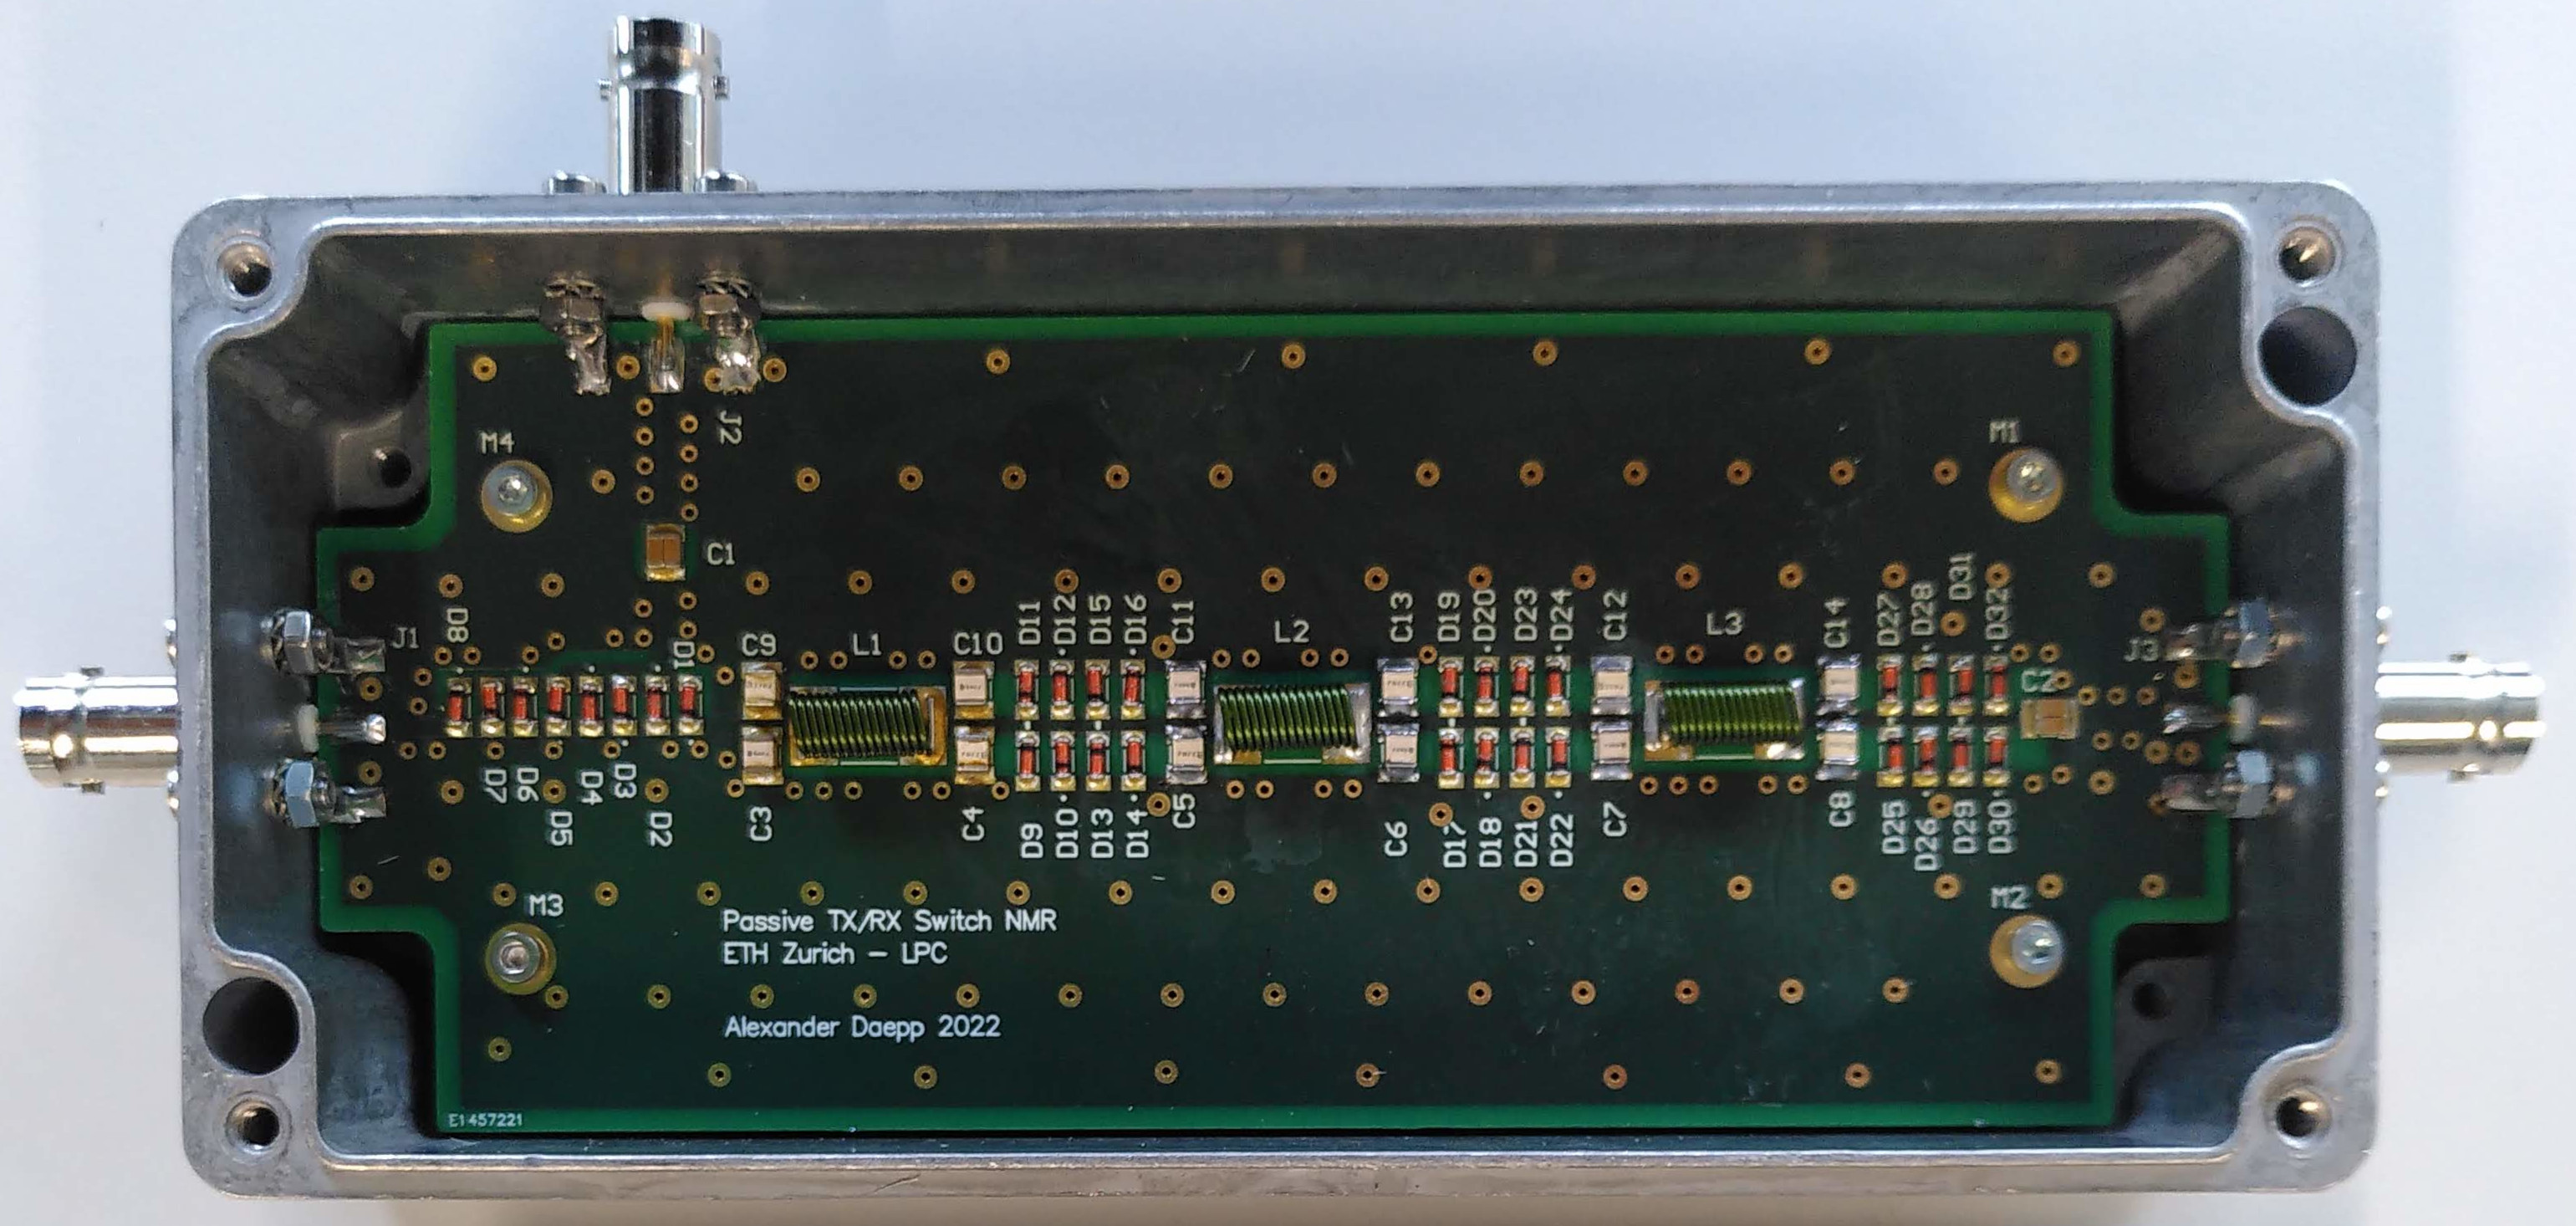
\includegraphics[width=\textwidth]{images/passive_tr_switch_assembled.jpg}
    \caption{\captiontitle{Passive \acrshort{rf} \acrshort{tr} switch} The power amplifier output would be connected on the left, the probe at the top and the low noise amplifier on the right.}
    \labfig{passive-switch}
\end{figure}

Unfortunately, due to the diode characteristics, the switch leaked at least \qty{7}{\deci\belm} of power which would be amplified by the low noise amplifiers to levels that could damage other electronics downstream. Additionally, during receive the power amplifier would generate more noise than anticipated and the diodes would conduct lower voltages than calculated, therefore adding noise to the received signal that was orders of magnitude larger than the actual signal. For these reasons, active switch designs were explored.

The active design of this kind of switch is called \acrfull{spdt} switch. A simple variant would be replacing the crossed diodes with biased PIN-diodes functioning effectively as \acrshort{rf} switches. This kind of \acrshort{spdt} switch is very fast and conceptually simple. Unfortunately, they typically also suffer from worse isolation at lower frequencies and have a higher power consumption due to the biasing compared to \acrshort{fet} switches. Biasing itself comes with its own challenges of mixing \acrshort{ac} and \acrshort{dc} usually using chokes and capacitors similar to the amplifier case. Lastly, many PIN diodes do not work at these low frequencies (\(<\qty{100}{\mega\hertz}\)) as the intrinsic region does not store enough charge for the negative half wave of the sinusoid.

Since the maximum power requirements are relatively low (see \refsec{poweramp}), integrated \acrshort{fet} switches become a viable solution. These work by simply connecting the individual branches using \acrshort{fet} transistors. Though slightly slower and less capable for higher power applications they provide very good isolation at these \enquote{low} frequencies in the \unit{\mega\hertz} range. They are commercially widely available for use in wireless infrastructure due to their broadband handling capabilities. Many variants exist that are already matched to \qty{50}{\ohm} and are absorptive in the off state. This helps with shortening the duration of the coil ringing and proves a safeguard for the power amplifier in case of misuse as most power amplifiers can be damaged when the output is open or unconnected like in a PIN-diode-based switch.

The Qorvo QPC6324 was therefore selected with a still acceptable insertion loss of \qty{0.9}{\deci\bel} and a high isolation of over \qty{60}{\deci\bel}, a \(P_{\qty{1}{\deci\bel}}\) of \qty{37}{\deci\belm}, \qty{50}{\ohm} matched, absorptive ports and \qty{3.6}{\volt} logic compatibility it is a good match for the circuit and easily controllable by the \acrfull{gpio} pins of the RedPitaya. No external circuitry or \acrshort{dc} blocking capacitors are needed, only a linear power supply to stabilize the input voltage and capacitances to limit the rise speed of the control lines were added to the \acrshort{pcb} design in \reffig{switch}.

\begin{figure}[hbt]
    \centering
    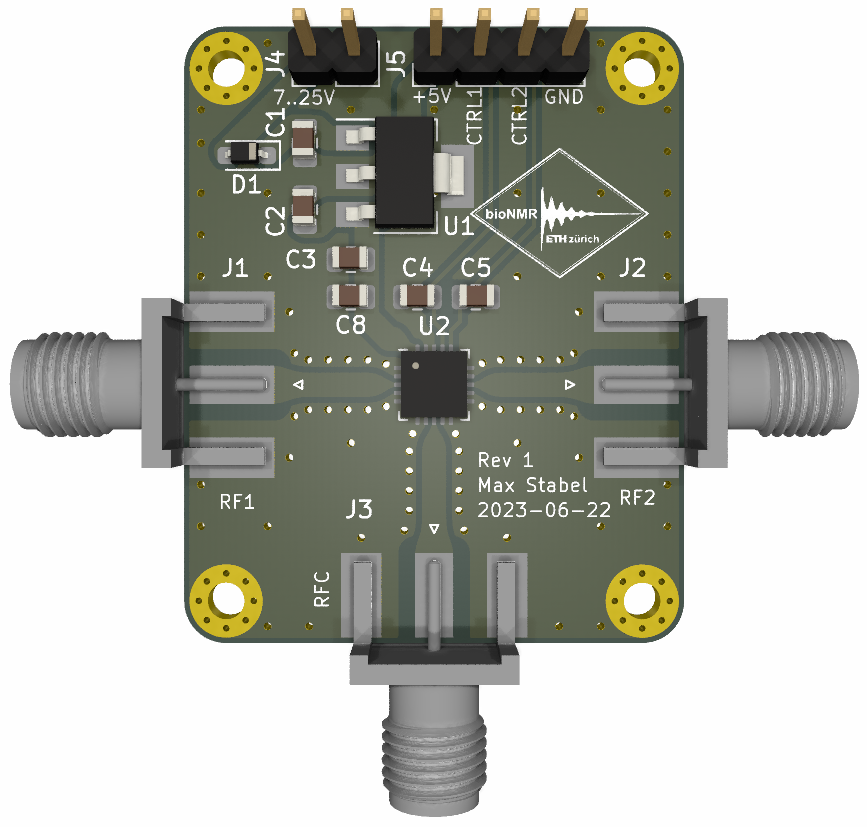
\includegraphics[width=\textwidth]{images/tr_switch.png}
    \caption{\captiontitle{\acrshort{rf} \acrshort{tr} switch} 3D rendering of the switch \acrshort{pcb} in KiCAD. The transmit and receive amplifiers are connected on the left and right, the probe at the bottom connector. The central part is a Qorvo QPC6324 \acrfull{spdt} switch. Above it is a linear power supply and connection pins for active switching and power supply.}
    \labfig{switch}
\end{figure}

\section{The probe}
\begin{marginfigure}[-4.5\baselineskip]
    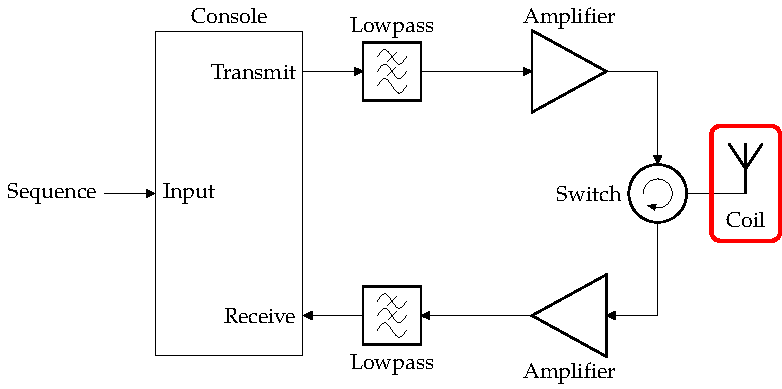
\includegraphics{block_diagram_highlight_coil.pdf}
    \labfig{block-diagram-coil}
\end{marginfigure}
To create the required \(B_1\) field to perturbate the population of spin states in the sample an \acrshort{rf} field needs to be generated\sidenote{while an \acrshort{rf} wave is generated as well, the far field is not used in the experiments and considered part of the loss.}. There are many possible designs for this conversion from the transmission line, the simplest being a solenoid coil used here. Myriads of parameters can be optimized in the probe including its type, length, diameter, number of windings, and consequently self-inductance and Q-factor as well. However, the solenoid is probably one of the best designs in terms of sensitivity for NMR, even though the inductance increases rapidly with the dimensions. It is best used for small samples and/or low fields \sidecite{mispelterNMRProbeheadsBiophysical2015} --- which is our case.

In addition the probe holder should position the sample correctly in the central homogeneous region of the magnet which is a \qty{6}{\milli\metre} diameter sphere. To this end a custom 3D printed probe holder was created with the solenoid coil mounted including the tuning and matching circuit.

The manufacturer of the magnet made a probe to guarantee the specifications of the magnet. This holder can be seen in \reffig{andrew-probe}. Unfortunately, the design files for the probe holder were not made available and the probe is significantly smaller than the space available in the magnet (\qty{50}{\milli\metre} x \qty{55}{\milli\metre} x \qty{9.5}{\milli\metre}), therefore correct positioning proved to be a challenge.

\begin{figure}[hbt]
    \centering
    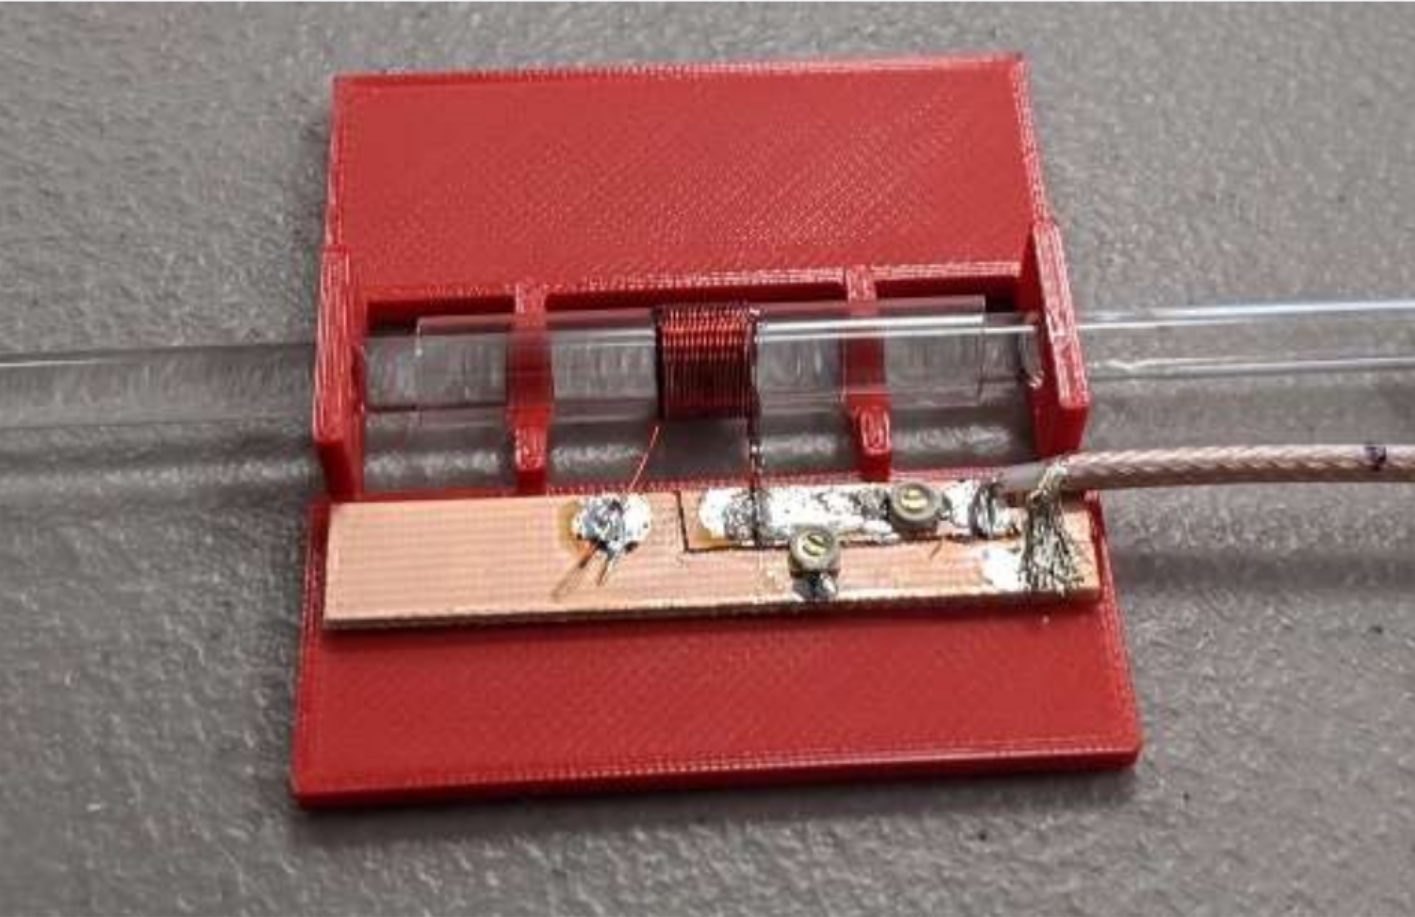
\includegraphics[width=\textwidth]{images/andrew-probe.png}
    \caption{\captiontitle{Manufacturer's probe holder and \acrshort{rf} coil with tuning and matching capacitors} The body was 3D printed and the circuit cut by hand.}
    \labfig{andrew-probe}
\end{figure}

The solenoid coil consists of \(\approx\qty{0.2}{\milli\metre}\) insulated copper wire wrapped around a clear plastic tube in 18 turns on a length of \qty{6}{\milli\metre} with a diameter of \qty{7.5}{\milli\metre} resulting in a theoretical self inductance of
\[
    L = \frac{\mu{}_0N^2A}{l} = \frac{\mu{}_0 \cdot{} 18^2 \cdot{} \pi{}  \cdot{} \frac{\qty{7.5}{\milli\metre}}{2}^2}{\qty{6}{\milli\metre}} = \qty{3.00}{\micro\henry}
\]
for a long air-filled coil. The self inductance of the coil inside the circuit (that is, with tuning and matching capacitors attached) was measured to be \qty{2.3}{\micro\henry} at \qty{1}{\kilo\hertz} with a PM6303 RCL meter.

The tuning and matching of the probe was performed outside the magnet with the resulting curve in \reffig{andrew-probe-tum}. The tuning and matching were very sensitive to the surroundings and should be redone inside the magnet when used for spectroscopic measurements.

\begin{figure}[hbt]
    \centering
    \includesvg[width=\textwidth]{images/probe_andrew_tum.svg}
    \caption{\captiontitle{The \(S_{11}\) coefficient of the manufacturer probe} On an x-scale from \qtyrange{20}{30}{\mega\hertz} and a logarithmic y-scale in \unit{\deci\bel}. Measured with a Rhode \& Schwarz ZNB 4 VNA.}
    \labfig{andrew-probe-tum}
\end{figure}

In an attempt to overcome the shortcomings of the manufacturers coil a larger version of it that fills the available space inside the magnet was created. This parameterized 3D model designed using openSCAD was then exported to a standard 3D model format, sliced and printed. The first print was done on a Prusa MK3S MMU2S with 0.3mm PLA on the \enquote{DRAFT} setting in roughly \qty{30}{\minute}. Due to small gaps at the connection joints of different parts it was printed again with a smaller print diameter of 0.2mm with the \enquote{QUALITY} setting which did not show any holes in \qty{1.25}{\hour} and can be found in \reffig{probe}. The full dimensions are \qty{70}{\milli\metre} x \qty{83.35}{\milli\metre} x \qty{10}{\milli\metre}, positioning the coil exactly in its center of the magnet.

\begin{figure}[hbt]
    \centering
    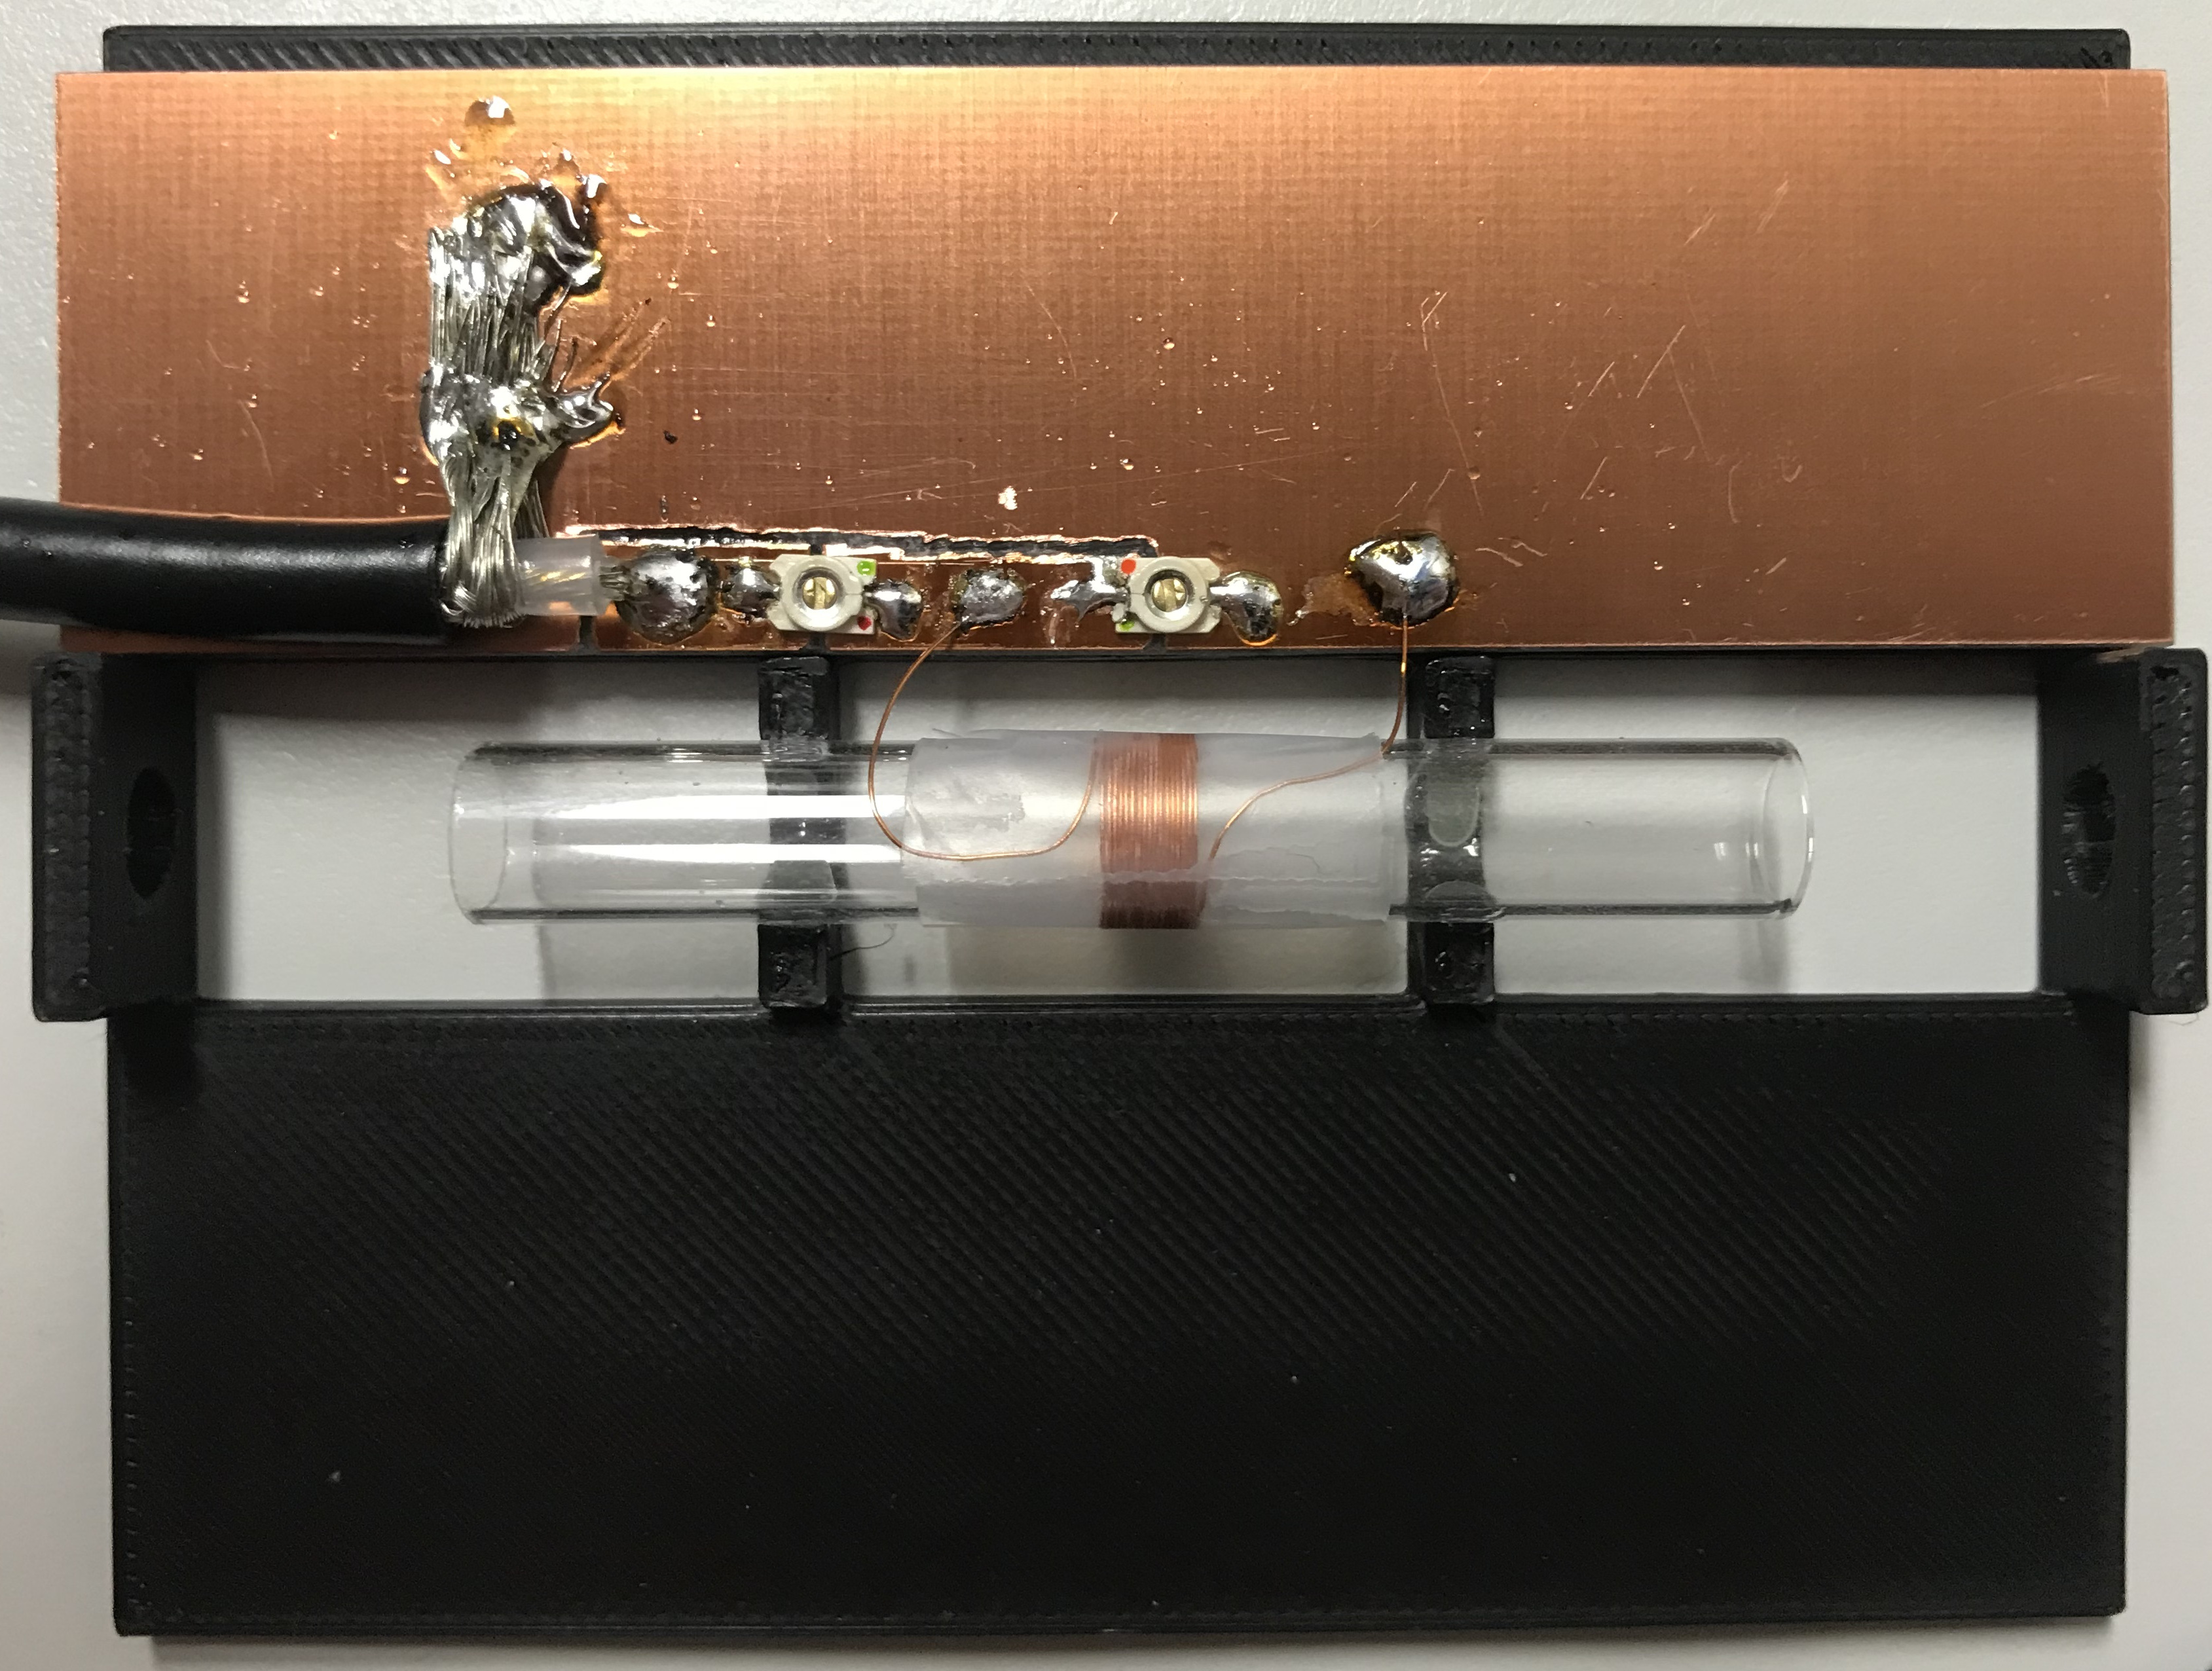
\includegraphics[width=\textwidth]{images/probe.jpg}
    \caption{\captiontitle{Probe holder and \acrshort{rf} coil with tuning and matching capacitors} The capacitors are tunable from \qtyrange{4.5}{20}{\pico\farad} of make JZ200HV. The coil has a diameter of \(d = \qty{7.5}{\milli\meter}\), wire diameter \(D = \qty{0.2}{\milli\meter}\) and \(n = \qty{18}{turns}\) on a length of \(l = \qty{4}{\milli\meter}\). It has a measured inductance of \(L_{\qty{1}{\mega\hertz}} = \qty{2.7}{\micro\henry}\) and a resistance of \(R_{\qty{1}{\mega\hertz}} = \qty{0.63}{\ohm}\). The body was 3D printed and the circuit cut by hand.}
    \labfig{probe}
\end{figure}

The coil was designed similarly to the manufacturer's probe as well. \qty{0.2}{\milli\metre} diameter insulated copper wire was wrapped 18 times around a \qty{7.5}{\milli\metre} glass tube on a length of \qty{4}{\milli\metre}. This results in a theoretical inductance for a long air-filled coil of \qty{4.5}{\micro\henry}. To reach a resonant frequency of \qty{25}{\mega\hertz} a tuning capacitance of about \qty{9}{\pico\farad} is thus needed in theory in an LC circuit. When measured with an HP4284 LCR-meter while resting on a styrofoam box an inductance of \qty{2.74}{\micro\henry} and a resistance of \qty{0.627}{\ohm} was measured at \qty{1}{\mega\hertz}. The difference can be attributed to stray capacitances of the connection wires, between the individual windings and the surroundings. The coil is also not long compared to the diameter --- a different model would be more accurate.

To estimate the coil behaviour closer to resonance frequency a resonant circuit was formed by connecting a \qty{10}{\pico\farad} capacitance to both ends end then measured using a pickup coil connected to a Rhode \& Schwarz ZNB4 \acrshort{vna}. The resonant frequency was estimated to be \qty{29.6}{\mega\hertz} using the well known LC resonance formula
\[
    f_{\text{res}} = \frac{1}{2\pi{}\sqrt{LC}}
\]
the inductance was calculated to be
\[
    L = \frac{1}{4\pi{}^2f_{\text{res}}^2C} = \frac{1}{4\pi{}^2 \cdot{} (\qty{29.6}{\mega\hertz})^2 \cdot{} \qty{10}{\micro\farad}} = \qty{2.89}{\micro\henry}
\] which is relatively close to the measured \qty{2.74}{\micro\henry} at \qty{1}{\mega\hertz}.

With the new inductance value, a capacitance of \(\approx{}\qty{14}{\pico\farad}\) is needed for resonance at \qty{25}{\mega\hertz}. To allow for tuning and matching of the circuit two variable capacitors with a range of \qtyrange{4.5}{20}{\pico\farad} was therefore chosen\sidenote{JZ200HV}. It is a high voltage, paramagnetic model. \reffig{probe} shows the complete probe. The completed probe was then tuned and matched outside the magnet with the results depicted in \reffig{probe-tum}.

\begin{figure}[hbt]
    \centering
    \includesvg[width=\textwidth]{images/probe_v1_tum.svg}
    \caption{\captiontitle{The \(S_{11}\) coefficient of the home-built probe} On an x-scale from \qtyrange{20}{30}{\mega\hertz} and a logarithmic y-scale in \unit{\deci\bel}. Measured with a Rhode \& Schwarz ZNB 4 VNA.}
    \labfig{probe-tum}
\end{figure}

Despite the seemingly better tuning and matching the signal of the home-built coil, the manufacture's probe gave better spectra, i.e. more lorentzian line shapes and a stronger signal. Qualitatively, the probe is less sensitive to stray capacitances and is better behaved inside the magnet, though this has not been quantified.

A lot more work can be done. The presented probe is utterly simple and functional, but by no means optimized. Different designs, parameters and configurations are to be explored. This includes saddle coils and variable pitch coils, but also approaches like distributed capacitances between the windings of the solenoid coil. For more consistency the winding patterns could be 3D printed as well.

Another important aspect is shielding of the probe which would provide more defined stray capacitances and reduce induced noise from the environment. Since the magnetic field is relatively homogenous even outside the small specified volume, a second coil with a fixed known sample could be included into the probe holder for locking purposes, simplifying the processing. Lastly the ability to tune and match the coil from the outside of the magnet would help greatly in usability.

\section{The low noise amplifier}

The low noise amplifier follows the same principles as the power amplifier. In \reffig{preamp} the signal travels from left to right first through a \qty{1.8}{\giga\hertz} low-pass filter as recommended by the \acrshort{lna} manufacturer to remove out of band frequencies that might cause distortions. Next is a set of crossed diodes decoupled with a capacitor to prevent \acrshort{dc}. They prevent any surges or leaked pulse to damage the amplifier that follows and clamp the voltage to \

The schematic can be found in the appendix \refsec{lna-schematic}.

The input


reference to martinos lab here

\begin{figure}[hbt]
    \centering
    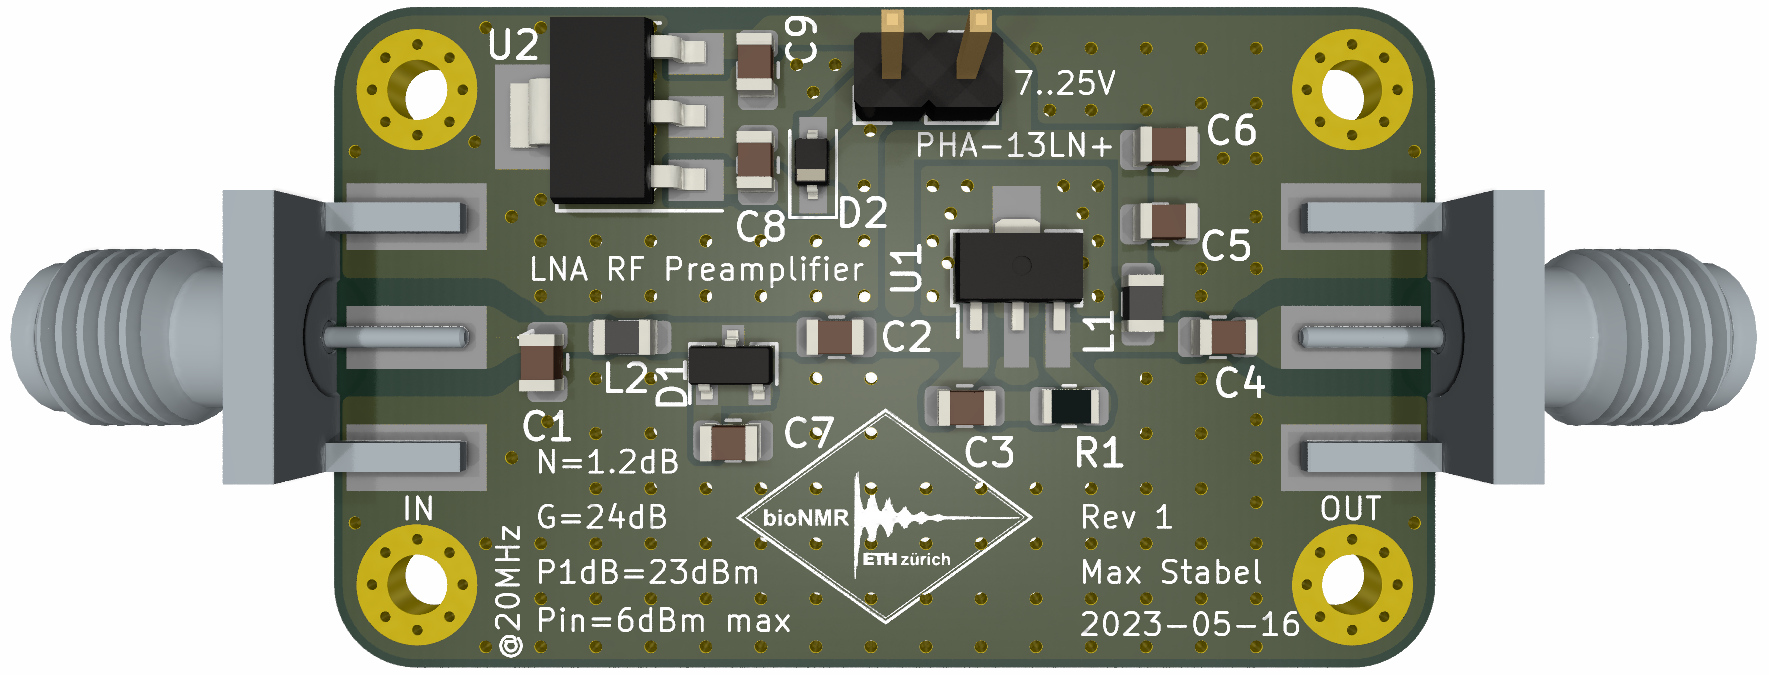
\includegraphics[width=\textwidth]{images/preamp.png}
    \caption{\captiontitle{The low noise amplifier} 3D rendering of the low noise amplifier \acrshort{pcb} in \gls{kicad}. The signal travels from left to right through a low-pass filter with \qty{1.8}{\giga\hertz} cut off frequency, a \qty{+5}{\deci\belm} clamping diode and the PHA-13LN+ low noise amplifier (\(G = \qty{24}{\deci\bel}, N = \qty{1.2}{\deci\bel}, P_{\qty{1}{\deci\bel} = \qty{23}{\deci\belm} @\qty{20}{\mega\hertz}}\)). The power is supplied by the onboard linear regulator at the top}
    \labfig{preamp}
\end{figure}

Basically the same as the power amplifier, just lower noise.

Mention input filter

Mention protection diodes

Mention oscillations

\section{The 32-channel current source}
building the power supply
\begin{figure}[hbt]
    \centering
    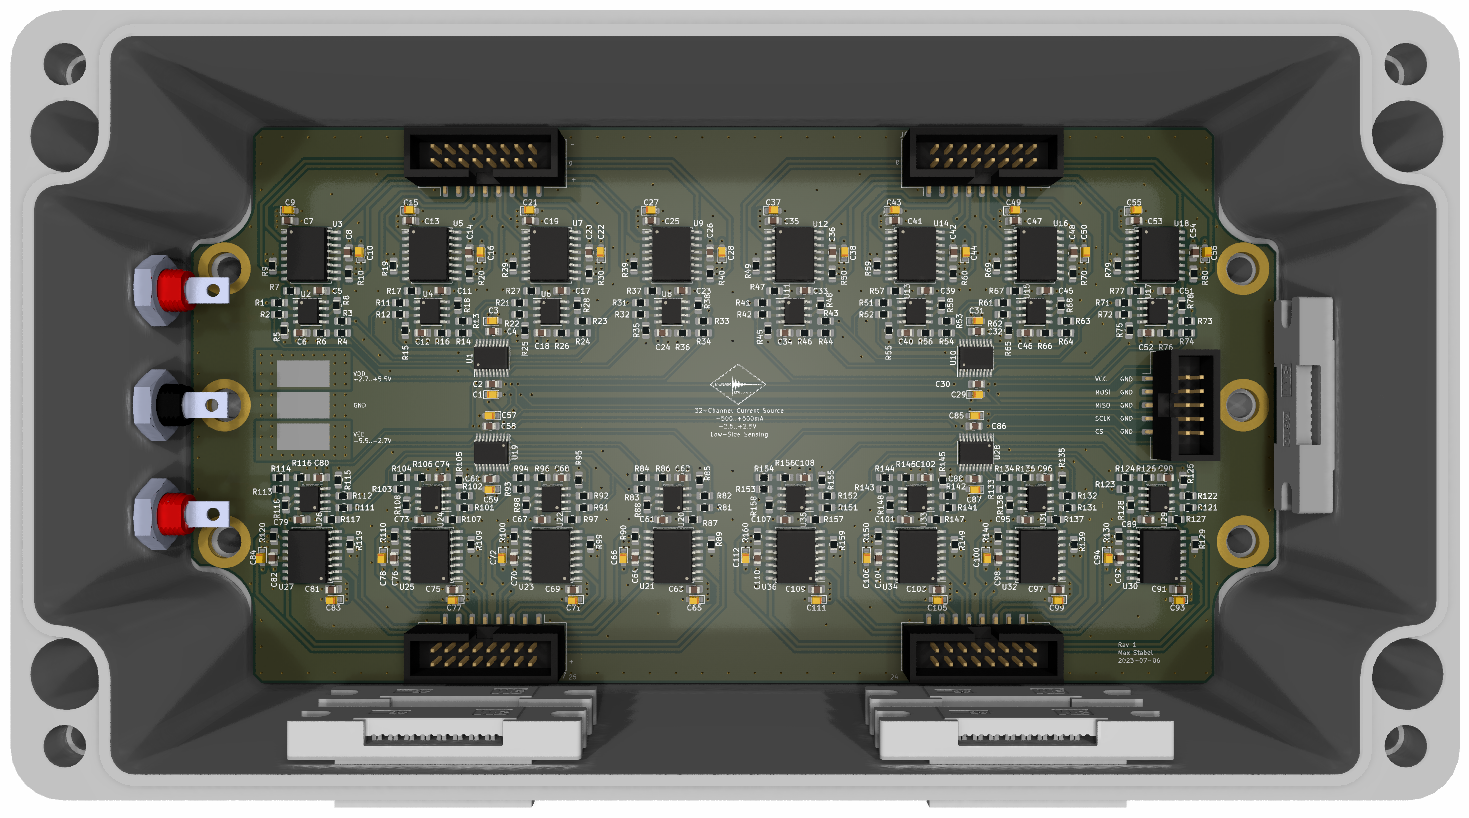
\includegraphics[width=\textwidth]{images/32-channel_current_source.png}
    \caption{\captiontitle{32-channel programmable current source.} 3D rendering of the current source \acrshort{pcb} in \gls{kicad}. The \acrshort{spi} interface is on the right, the power connectors on the left and the 32 output channels on the top and bottom of the \acrshort{pcb}. It consists of 4 8-channel \acrshort{adc}s (AD5676R) setting a voltage that is converted to a constant current by two \acrshort{opamp}s: LMV358 for signal scaling and shifting and TCA0372 for the constant current source.}
    \labfig{current-source}
\end{figure}

\section{The magnet}
\labsec{magnet}
The magnet was built by SABR Enterprises, LLC with a homogenous volume of \qty{100}{\micro\litre} using a \qty{5}{\milli\metre} NMR tube. It has a field strength of \qty{0.6}{\tesla}/\qty{25}{\mega\hertz} with a homogeneity of at least \qty{0.1}{\partspermillion} inside the homogenous volume with the magnetic ink shims and active electronic shimming performed by NuevoMR, LLC\sidenote{spherical harmonic fields of order 1-4 (except \(XY(X^2-Y^2)\))}. A simple two-dipole setup is employed due to the ease of construction and shimming. The schematic can be found in the appendix \refsec{magnet-schematic}.

A Halbach array --- the so-called NMR Mandhala --- was considered as well. While the achievable field strengths of \qtyrange{0.5}{2}{\tesla} \sidecite{blumichCompactNMR2014} are sufficient, the initially achievable line width of \qty{700}{\partspermillion} \cite{raichDesignConstructionDipolar2004} (without shims) magnets is not\sidenote{The chosen dipole magnet achieves a homogeneity \qty{4.7}{\partspermillion} without active shims}. This can be compensated by further passive and active shimming, at the expense of adding complexity to the design. The shimming of Mandhala magnets is still an ongoing research topic, see for example \sidecite{danieliSmallMagnetsPortable2010}, \sidecite{parkerShimmingHalbachMagnets2016} or \sidecite{wangDesignShimmingMethod2022} paper. This design is worth investigating further in the future promising low sub-kg weighta as well as price reductions --- also considering the current price point for the dipole magnet of \approx \qty{9}{kCHF}.

For the material, temperature-compensated samarium cobalt (SmCo TC, EC 2:17-TC16) with a reversible temperature coefficient (RTC) of \qty{-0.001}{\%\per\kelvin} was chosen. The more common and cheaper Neodymium is more temperature sensitive with an RTC of around \qty{-0.1}{\%\per\kelvin}. Due to the low field, multiple scans will likely be required for at least some NMR measurements, exasperating the undesirable effect of a field drift over longer periods.

\section{The software}
\labsec{software}
The low-level \gls{marcos} software has been introduced in \refsec{console}. The \gls{marcos} client library sends \enquote{msgpack} formatted data from the PC to the C++ server running on the console, which handles sequence compilation and stream management with the \acrshort{fpga}. Around this client client library a simple interface for sending and receiving pulse sequences has been built.

Using \enquote{nmrglue} \sidecite{helmusNmrglueOpenSource2013} it is possible to save the data in the popular NMRPipe \sidecite{delaglioNMRPipeMultidimensionalSpectral1995} data format. This could easily be extended in the future to include for example the relatively new nmrML\sidecite{schoberNmrMLCommunitySupported2018} open data standard or the older JCAMP-DX \sidecite{mcdonaldJCAMPDXStandardForm1988} format. The software adds simple processing and analysis shortcuts for 1D NMR spectra to facilitate easy and quick inspection of the data. This includes plotting, fourier transform, automatic phase correction, scale conversions, peak picking and single peak as well as spectra fitting.

The usage of the software is described further in \refch{complete}. Additional information can be found inside the repository including example scripts, demonstration notebooks, \acrshort{cli} documentation and an \acrshort{api} reference.
